% Este archivo es parte de la memoria del proyecto fin de carrera
% de Manuel López Urbina. Protegida bajo la licencia GFDL.
% Para más información, la licencia completa viene incluida en el
% fichero fdl-1.3.tex

% Copyright (C) 2018 Manuel López Urbina
\newpage

\chapter{Conceptos básicos}
\label{chap:conceptos-básicos}


En el presente capítulo se recogen aquellos conceptos, definiciones, protocolos y diferentes aspectos que resultan de especial interés y que ayudarán a la comprensión de los diferentes puntos tratados en el resto de 
la memoria sin profundizar demasiado en detalles técnicos.\\

Todos estos conceptos se encuentran estrechamente ligados con tecnologías de la comunicación y transmisión de información y señales. Además de una sección destinada a los sensores, recogiendo sus 
características y tipos existentes a modo general.\\


\section{Telemetría}
\label{def:telemetria}

La telemetría es una tecnología destinada la medición de magnitudes físicas de manera remota para un posterior envío de la información hacia un sistema que actúa como operador. La palabra telemetría
procede de las palabras griegas τῆlε (tele), la cual significa distancia, y la palabra μετρον (metron), que indica medida \cite{book:telemetria}.\\

El envío de información se realiza típicamente mediante comunicación inalámbrica, característica fundamental de estos sistemas aunque también se pueden emplear otros medios 
como redes de computadoras, fibra óptica, GSM, etc. Los sistemas de telemetría reciben las órdenes o instrucciones desde un sistema externo que hace las 
funciones de control.\\


\begin{figure}[H]
  \begin{center}
    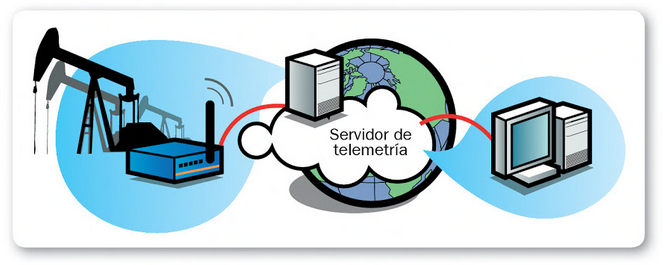
\includegraphics[scale=0.4]{imagenes/telemetria.png}
  \end{center}
  \label{fig:telemetria}
 \caption{Esquema básico de comunicación en un sistema de telemetría.}
\end{figure}



\subsection{Aplicaciones}

La telemetría se utiliza tanto en sistemas simples como en sistemas de muy elevada complejidad. Estos sistemas pueden ser de muy diversa índole como por ejemplo, naves espaciales,
plantas químicas, redes de suministro (agua, gas, electricidad...) entre muchos otros. Dado que la telemetría posibilita la monitorización automática y el registro de las mediciones
permiten el envío de alertas o alarmas al centro de control con el fin de que el funcionamiento sea seguro y eficiente.\\

Por ejemplo, las agencias espaciales como la NASA, la UK Space Agency, la ESA y otras, utilizan sistemas de telemetría y de telecontrol para operar con satélites y naves espaciales,
o en la Fórmula 1 donde se utilizan para la medición de las condiciones de la pista y transmitir al piloto información relevante para bajar sus tiempos por vuelta. En las fábricas donde
el monitoreo de variables que afecten a la producción permitirá elaborar sistemas de mayor eficiencia energética reduciendo los costes.\\

\section{Sensor}
\label{sec:sensor-definicion}

Un sensor es un dispositivo módulo o subsistema que permite cuantificar una variable física cuyo propósito es detectar eventos o cambios en su entorno y
enviar la información a otros componentes electrónicos, con frecuencia un procesador de computadora. Un sensor siempre es utilizado en combinación con 
otros dispositivos electrónicos, para su posterior procesamiento, transmisión, activación de una acción, etc. \cite{book:sensoresyactuadores}. \\


\subsection{clasificación}

% https://books.google.es/books?id=CuoXCd6ZZqwC&pg=PR9&dq=sensores+clasificacion&hl=es&sa=X&ved=0ahUKEwiJ7vChrbvdAhUFXxoKHdbdBFMQ6AEITjAH#v=onepage&q=sensores%20clasificacion&f=false

Dada la gran cantidad de sensores existentes resulta necesario aplicar una clasificación con la finalidad de comprender mejor su naturaleza y funcionamiento. Los sensores se pueden 
clasificar de diversas formas según los distintos criterios atendidos \cite{book:guiapracticasensores}:\\

\begin{figure}[H]
  \begin{center}
    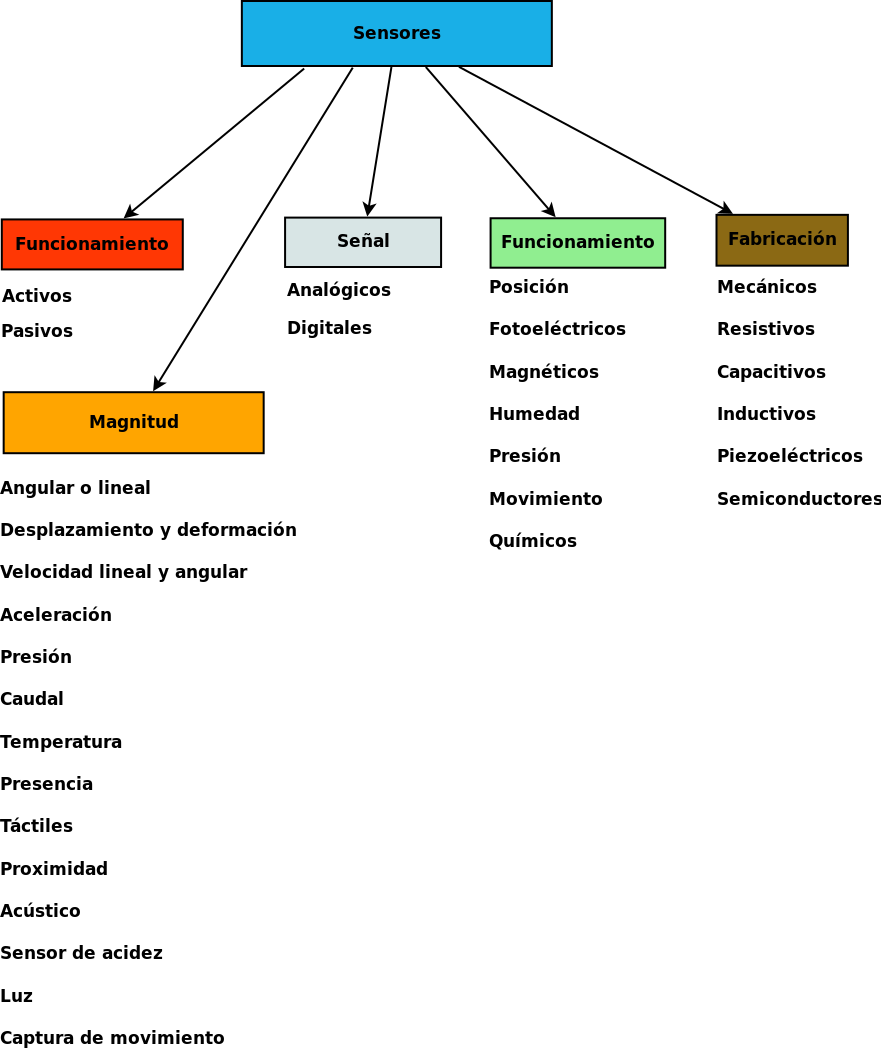
\includegraphics[scale=0.4]{diagramas/sensores_clasificacion.png}
  \end{center}
  \label{fig:clasificacion_sensores}
 \caption{Esquema de clasificación de los sensores según criterio.}
\end{figure}

\subsubsection{Atendiendo a su funcionamiento:}
\begin{itemize}
 \item \textbf{Activos:} Requieren de una fuente externa de energía de la que recibir alimentación de corriente para su funcionamiento.
 \item \textbf{Pasivos:} No requieren de una fuente de energía externa, sino que las propias condiciones medioambientales son suficientes para que funcionen según su cometido.
\end{itemize}

\subsubsection{Atendiendo a las señales que proporcionan:}

\begin{itemize}
 \item \textbf{Analógicos:} Proporcionan la información mediante una señal analógica (tensón, corriente), es decir, que pueden tomar infinidad de valores entre un mínimo y
 un máximo.
 \item \textbf{Digitales:} Proporcionan la información mediante una señal digital que puede ser un 0 o un 1 lógicos, o bien un código de bits.
\end{itemize}

\begin{figure}[H]
    \centering
    \begin{subfigure}[b]{0.4\textwidth}
        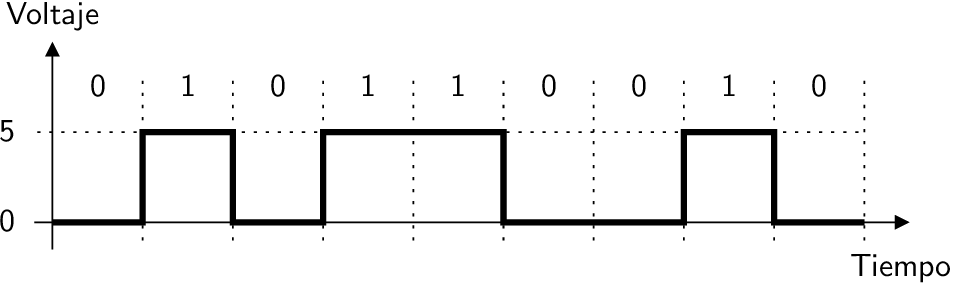
\includegraphics[width=\textwidth]{imagenes/senal_digital.png}
        \caption{Señal digital}
        \label{fig:gull}
    \end{subfigure}
    \begin{subfigure}[b]{0.26\textwidth}
        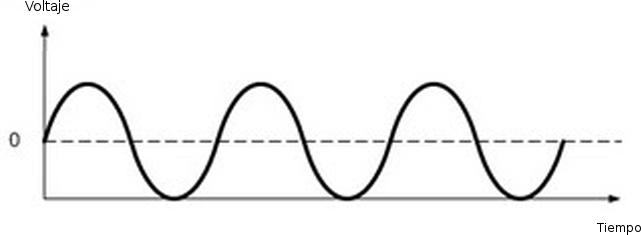
\includegraphics[width=1.19\textwidth]{imagenes/senal_analogica.png}
        \caption{Señal analógica}
        \label{fig:tiger}
    \end{subfigure}
    \caption{Ejemplos de señal digital y analógica.}\label{fig:animals}
\end{figure}

\subsubsection{Atendiendo a la naturaleza de su funcionamiento:}

\begin{itemize}
 \item \textbf{Posición:} Son aquellos que experimentan variaciones en función de la posición que ocupan en cada instante los elementos que lo componen.
 \item \textbf{Fotoeléctricos:} Son aquellos que experimentan variaciones en función de la luz que incide sobre los mismos.
 \item \textbf{Magnéticos:} Son aquellos que experimentan variaciones en función de la temperatura del lugar donde están ubicados.
 \item \textbf{Humedad:} Son aquellos que experimentan variaciones en función del nivel de humedad existente en el medio en el que se encuentran.
 \item \textbf{Presión:} Son aquellos que experimentan variaciones en función de la presión a la que son sometidos.
 \item \textbf{Movimiento:} Son aquellos que experimentan variaciones en función de los movimientos a los que son sometidos.
 \item \textbf{Químicos:} Son aquellos que experimentan variaciones en función de los agentes químicos externos que pudieran incidir sobre ellos.
\end{itemize}

\subsubsection{Atendiendo a los elementos utilizados en su fabricación:}

\begin{itemize}
 \item \textbf{Mecánicos:} Son aquellos que utilizan contactos mecánicos que se abren o cierran.
 \item \textbf{Resistivos:} Son aquellos que utilizan en su fabricación elementos resistivos.
 \item \textbf{Capacitivos:} Son aquellos que emplean condensadores.
 \item \textbf{Inductivos:} Son aquellos que emplean bobinas.
 \item \textbf{Piezoeléctricos:} Son aquellos que emplean cristales como el cuarzo.
 \item \textbf{Semiconductores:} Son aquellos que emplean materiales Semiconductores.
\end{itemize}


\subsubsection{Atendiendo a la magnitud}

\textbf{Posición angular o lineal:}
\begin{itemize}
 \item Potenciómetro
 \item Encoder
\end{itemize}

\textbf{Desplazamiento y deformación:}
\begin{itemize}
 \item Gala extensiométrica
 \item Magnetoestrictivos
 \item LVDT
\end{itemize}

\textbf{Velocidad lineal y angular:}
\begin{itemize}
  \item     Dinamo tacométrica
  \item     Encoder
  \item     Inclinometros
  \item     RVDT
  \item     Giróscopio
\end{itemize}

\textbf{Aceleración:}
\begin{itemize}
  \item     Acelerómetro
  \item     Fuerza y par (deformación)
  \item     Galgas extensiométrica
  \item     Triaxiales
\end{itemize}

\textbf{Presión:}
\begin{itemize}
  \item     Membranas
  \item     Piezoeléctricos
  \item     Manómetros digitales
\end{itemize}

\textbf{Caudal:}
\begin{itemize}
  \item     Turbina
  \item     Magnético
\end{itemize}

\textbf{Temperatura:}
\begin{itemize}
  \item     Termopar
  \item     RTD
  \item     Termistor NTC
  \item     Termistor PTC
  \item     Bimetal
\end{itemize}

\textbf{Presencia:}
\begin{itemize}
  \item     Inductivos
  \item     Capacitivos
  \item     Ópticos
\end{itemize}

\textbf{Táctiles:}
\begin{itemize}
  \item     Matriz de contactos
  \item     Piel artificial
\end{itemize}

\textbf{Proximidad:}
\begin{itemize}
  \item     Capacitivo
  \item     Inductivo
  \item     Fotoeléctrico
\end{itemize}

\textbf{Acustico:}
\begin{itemize}
  \item     Micrófono
\end{itemize}

\textbf{Sensor de acidez:}
\begin{itemize}
  \item     ISFET
\end{itemize}

\textbf{Luz:}
\begin{itemize}
  \item     Fotodiodo
  \item     Fotoresistencia
  \item     Fototransistor
\end{itemize}

\textbf{Captura de movimiento:}
\begin{itemize}
  \item     Sensor inercial
\end{itemize}

Algunas magnitudes pueden calcularse mediante la medición y cálculo de otras, por ejemplo, la velocidad de un móvil puede calcularse a partir de la integración numérica de su 
aceleración. La masa de un objeto puede conocerse mediante la fuerza gravitatoria que se ejerce sobre él en comparación con la fuerza gravitatoria ejercida sobre un objeto de 
masa conocida. \\

\subsection{Atendiendo a los errores de medición}

La mayoría de los sensores tienen una función de transferencia lineal. La sensibilidad se define entonces como la relación entre la señal de salida y la propiedad medida. 
Por ejemplo, si un sensor mide la temperatura y tiene una salida de voltaje, la sensibilidad es constante con las unidades [V / K]. La sensibilidad es la pendiente de la función 
de transferencia. La conversión de la salida eléctrica del sensor (por ejemplo V) a las unidades medidas (por ejemplo K) requiere dividir la salida eléctrica por la pendiente 
(o multiplicar por su recíproco). Además, con frecuencia se agrega o resta una compensación. Por ejemplo, se debe agregar -40 a la salida si la salida de 0 V corresponde a la 
entrada de -40 \textdegree C.\\

\begin{itemize}
 \item Sensibles a la propiedad medida.
 \item Insensibles a cualquier otra propiedad que pueda encontrarse en su aplicación.
 \item No influyen en la propiedad medida.
\end{itemize}

Para que una señal de sensor analógico sea procesada o utilizada en un equipo digital, necesita convertirse en una señal digital, utilizando un convertidor de analógico a 
digital añadiendo un posible error a la salida.\\



\subsection{Características de los sensores}

El sensor  ideal  sería  aquel  en  que  la  relación  entre la magnitud de entrada y la 
magnitud de salida fuese proporcional y de respuesta instantánea e idéntica para todos los elementos de un mismo tipo. \\

Sin  embargo, la respuesta real de los sensores  nunca  es del todo lineal, tiene un rango  limitado  de  validez que  suele  estar afectada por perturbaciones del entorno exterior además de tener un cierto retardo en la respuesta. \\

Las características de los sensores se pueden agrupar en dos grandes bloques en cuanto a sus característica se refiere:\\

\begin{enumerate}
 \item \textbf{Características estáticas}, que describen la actuación del sensor en régimen permanente o 
con cambios muy lentos de la variable a medir. \\
 \item \textbf{Características dinámicas}, que describen el comportamiento del sensor en régimen transitorio.\\
\end{enumerate}


\begin{figure}[H]
  \begin{center}
    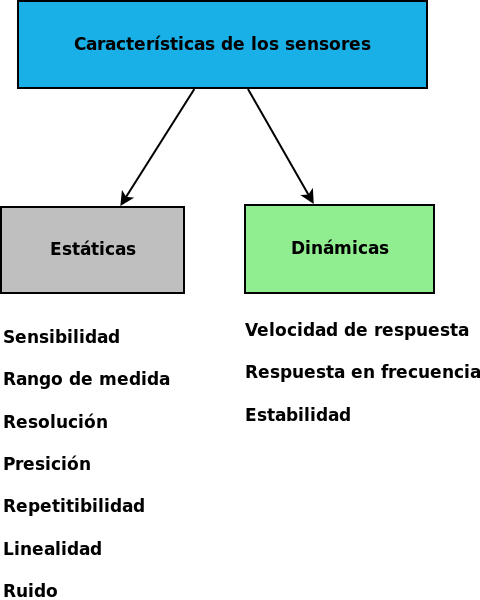
\includegraphics[scale=0.4]{diagramas/sensores_propiedades.png}
  \end{center}
  \label{fig:telemetria}
 \caption{Esquema clasificatorio de las características estáticas y dinámicas de los sensores.}
\end{figure}


\subsubsection{Estáticas}

Instrumentos basados en la medición de parámetros estables, es decir, mediciones de valores que no presenten variaciones bruscas en su magnitud de salida.\\

\textbf{Sensibilidad:}\\

La sensibilidad de un sensor indica cuánto cambia la salida del sensor cuando cambia la cantidad de entrada que se mide. Por ejemplo, si el mercurio en un termómetro se mueve
1 cm cuando la temperatura cambia en 1 grado, la sensibilidad es 1 cm/C (es básicamente la pendiente Dy/Dx asumiendo una característica lineal).\\

\textbf{Rango de medida:}\\

El  conjunto  de  valores  que  puede  tomar  la  señal  de  entrada comprendidos  entre  el  máximo  y  el  mínimo  detectados  por  el  sensor  con  una  tolerancia 
de error aceptable. \\

\textbf{Resolución:} \\

Indica la capacidad del sensor para discernir entre valores muy próximos de la variable de entrada. Indica que variación de la señal de entrada produce una variación detectable en la señal de salida. \\

\textbf{Presición:}\\

Define la variación  máxima entre la salida real obtenida y la salida teórica dada como patrón para el sensor. \\

\textbf{Repetitibilidad:}\\

Indica la  máxima  variación  entre  valores  de  salida  obtenidos al  medir varias veces la misma entrada con el mismo sensor y en idénticas condiciones 
ambientales.\\

\textbf{Linealidad:}\\

Un  transductor  es  lineal  si  existe  una  constante  de  proporcionalidad  única 
que relaciona los incrementos de la señal de salida con los respectivos incrementos de la 
señal de entrada en todo el rango de medida. \\

\textbf{Ruido:}\\

Cualquier perturbación aleatoria del propio sistema de medida que afecta la señal 
que se quiere medir. \\

\subsubsection{Dinámicas}

Puede ocurrir que la cantidad bajo medición sufra una variación en un momento determinado y por lo tanto es necesario que conozcamos el comportamiento dinámico del instrumento 
cuando sucedan estas variaciones.\\

\textbf{Velocidad de respuesta:}\\

Mide la capacidad del sensor para que la señal de salida siga sin retraso las variaciones de la señal de entrada. \\

\textbf{Respuesta en frecuencia:}\\

Mide la capacidad del sensor para seguir las variaciones de la 
señal  de  entrada  a  medida  que  aumenta  la  frecuencia,  generalmente  los  sensores 
convencionales presentan una respuesta del tipo paso bajo.\\

\textbf{Estabilidad:}\\

Indica  la  desviación  en  la  salida  del  sensor  con  respecto  al  valor  teórico 
dado,  al  variar  parámetros  exteriores  distintos  al  que  se  quiere  medir  (condiciones 
ambientales, alimentación, etc.). \\


\section{Transmisión y comunicación}
\label{sec:transmisión}

Se denomina \emph{transmisión} como el proceso de transporte de una señal de un lugar a otro y \emph{comunicación} como el intercambio entre dos entes mediante una transmisión, los cuales son capaces de
interpretar la información circundante entre ellos y en el cual existen un conjunto de reglas definidas, los protocolos\footnote{Protocolo: reglamento o serie de instrucciones que se fijan por tradición o por convenio. },
que rigen el proceso.

\section{Socket}
\label{sec:def-socket}

\emph{Socket}, o también conocido como conector, designa un concepto abstracto mediante el cual dos programas, generalmente situados en computadoras distintas, pueden intercambiar cualquier flujo de datos
de manera fiable y ordenada.\\

La comunicación a través de una red de ordenadores es una tarea compleja en la que para resolverla se ha empleado un enfoque de diseño por capas, pudiéndose hablar por tanto de una arquitectura 
o pila de protocolos donde cada capa utiliza servicios (funciones) de la capa inferior y ofrece servicios a la capa superior. \\

El modelo de referencia para la comunicación de ordenadores es el denominado modelo de Interconexión de Sistemas Abiertos OSI ( Open Systems Interconection ), el cual queda descrito
en la sección \ref{sec:modelo-osi} junto con la localización de los sockets en dicho modelo.\\

El término \emph{socket} es también usado como el nombre de una interfaz de programación de aplicaciones (API) para la familia de protocolos de red TCP/IP \footnote{ TCP/IP es un conjunto de protocolos que
permiten la comunicación entre los ordenadores pertenecientes a una red. La sigla TCP/IP significa Protocolo de control de transmisión/Protocolo de Internet. Proviene de los nombres de dos protocolos 
importantes incluidos en el conjunto TCP/IP, es decir, del protocolo TCP y del protocolo IP. }, provista usualmente por el sistema operativo.\\

Los sockets constituyen el mecanismo para la entrega de paquetes de datos provenientes de la tarjeta de red a los procesos o hilos apropiados. Un socket queda definido por un par de direcciones IP local
y remota, un protocolo de transporte y un par de números de puerto local y remoto.\\

Cuando se habla de dirección y puerto local/remoto, se sobreentiende que nos referimos a dos procesos (cliente/servidor o nodo/nodo) ya que ambas direcciones IP y puerto pueden coincidir para el intercambio de información entre procesos dentro de una misma máquina
y; además, la comunicación puede ser perfectamente bidireccional, asumiendo que el par que la inicia es el cliente y su contrapartida un servidor pero pudiendo ejercer de forma ambivalente ambas partes.\\


\section{WebSocket}
\label{sec:def-websocket}

Comprendido previamente el concepto de \emph{socket} descrito en el punto \ref{sec:def-socket}, definimos  \emph{Websocket} como una tecnología que proporciona un canal de comunicación bidireccional y full-duplex 
\footnote{Full Duplex: definido como la capacidad de transmisión y recepción en ambas direcciones al mismo tiempo. } utilizada por cualquier aplicación cliente/servidor.\\


La API de WebSocket está siendo normalizada por el W3C, mientras que el protocolo WebSocket ya fue normalizado por la IETF\footnote{Internet Engineering Task Force (IETF) (en español, Grupo de Trabajo de Ingeniería de Internet)
es una organización internacional abierta de normalización, que tiene como objetivos el contribuir a la ingeniería de Internet, actuando en diversas áreas, como transporte, encaminamiento, seguridad.
Se creó en los Estados Unidos, en 1986. Es mundialmente conocido porque se trata de la entidad que regula las propuestas y los estándares de Internet, conocidos como RFC.} como el RFC 6455.\\

Debido a que las conexiones TCP comunes sobre puertos diferentes al 80 son habitualmente bloqueadas por los administradores de redes, el uso de esta tecnología proporcionaría una solución
a este tipo de limitaciones proveyendo una funcionalidad similar a la apertura de varias conexiones en distintos puertos, pero multiplexando diferentes servicios WebSocket sobre un único
puerto TCP a costa de una pequeña sobrecarga del protocolo.\\

\section{La arquitectura TCP/IP y el modelo OSI}
\label{sec:modelo-osi}

En 1977 la Organización Internacional de Estandarización ( Internacional Standards Organization , ISO) estableció un subcomité encargado de diseñar una arquitectura de
comunicación. El resultado fue el modelo de referencia para la Interconexión de Sistemas Abiertos OSI ( Open Systems Interconection ). Dicho modelo define una arquitectura de
comunicación estructurada en siete niveles verticales. Dicho modelo es utilizado como base teórica para el desarrollo de la arquitectura TCP/IP, la cual está compuesta por una serie de capas
o niveles en los que se encuentran los protocolos que implementan las funciones necesarias para la comunicación entre dos dispositivos en red.\\

Siendo, por tanto, el modelo OSI el empleado en el estudio de las redes de datos y el modelo o arquitectura TCP/IP como un modelo real
empleado es las redes actuales.\\

La Figura \ref{diagram:modelo-osi-tcp} representa los distintos niveles o capas de los modelos OSI y TCP/IP y la disposición de los sockets dentro de ellos.\\

\begin{figure}[H]
  \begin{center}
    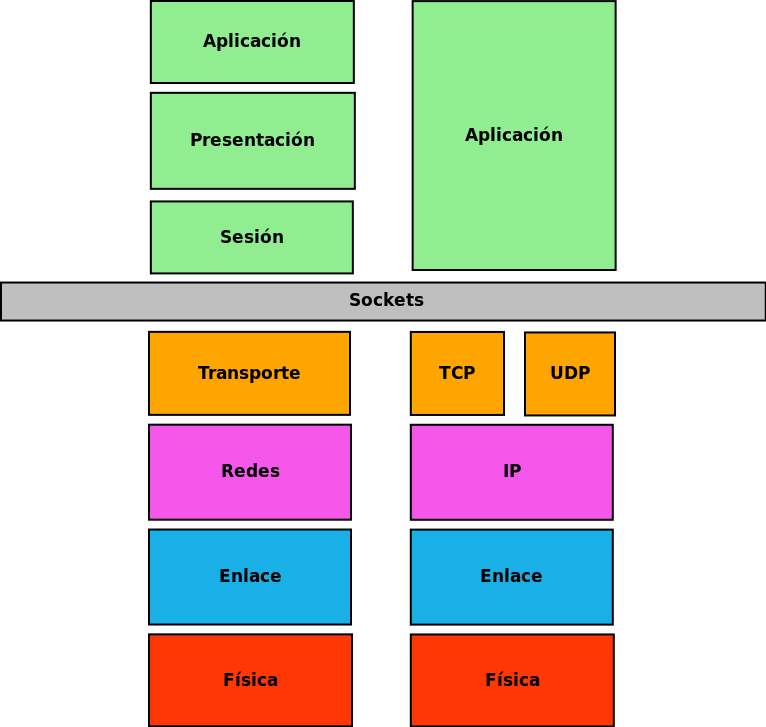
\includegraphics[scale=0.4]{diagramas/modelo-capas.png}
  \end{center}
  \caption{ Representación de los modelos de capas o niveles OSI y TCP/IP.}
  \label{diagram:modelo-osi-tcp}
\end{figure}

\section{Streaming}
\label{sec:def-streaming}

La retransmisión, streaming o también denominado transmisión, es la distribución digital de contenido multimedia a través de una red de computadoras, 
de manera que el usuario \emph{``consume''} el producto medida que es descargado. La palabra retransmisión se refiere a una corriente continua la cual fluye sin interrupción,
habitualmente audio o vídeo.\\

Este tipo de tecnología funciona mediante un buffer de datos que va almacenando el flujo de descarga en la estación del usuario para inmediatamente mostrarle el material descargado. Esto se contrapone al mecanismo de
descarga de archivos, que requiere que el usuario descargue los archivos por completo para poder acceder al contenido.\\

Como requisito fundamental, la retransmisión requiere de una conexión por lo menos de igual ancho de banda que la tasa de transmisión del servicio. Los servicios de streaming en 
Internet se popularizaron entre los años 2009 y 2010, cuando las compañías de telecomunicaciones pudieron ofrecer del suficiente ancho de banda para utilizar estos servicios
en el hogar a un coste relativamente asequible.

\section{Comunicación serie}

La comunicación serie o comunicación secuencial, en telecomunicaciones e informática, es el proceso de envío de datos de un bit a la vez, de forma secuencial, sobre un canal
de comunicación o un bus.\\

En cambio, en la “comunicación en paralelo” todos los bits de cada símbolo se envían al mismo tiempo, y por ello debe haber al menos tantas líneas de comunicación como bits tenga
la información a transmitir.\\

\subsection{Características}

La ventaja de la comunicación serie es que necesita un número más pequeño de líneas de transmisión que una comunicación paralela que transmita la misma información. Esta última
necesita tantas líneas de transmisión como la cantidad de bits que componen la información, mientras que la primera se puede llevar a cabo con una sola línea de transmisión. Por otra parte,
surgen una serie de problemas en la transmisión de un gran número de bits en paralelo, como los problemas de interferencia o desincronización.\\

A la misma frecuencia de transmisión, la comunicación paralela tiene un mayor rendimiento. La comunicación serie tiene que compensar esta debilidad con una frecuencia más alta.\\

Ejemplos:\\

\begin{itemize}
 \item Código Morse
 \item Ethernet
 \item Fibre Channel
 \item FireWire
 \item I²C
 \item MIDI
 \item PCI Express
 \item RS-232
 \item RS-485
 \item Serial ATA
 \item Serial Peripheral Interface
 \item Universal Serial Bus
\end{itemize}

\section{PWM}

La modulación de ancho de pulso (PWM) o la modulación de duración de pulso (PDM) es una técnica de modulación utilizada para codificar un mensaje en una señal de pulso. 
Aunque esta técnica de modulación puede utilizarse para codificar información para la transmisión, su uso principal es permitir el control de la potencia suministrada a los
dispositivos eléctricos, especialmente a cargas inerciales tales como motores. Además, PWM es uno de los dos principales algoritmos utilizados en los cargadores de baterías solares
fotovoltaicas, el otro es el seguimiento del punto de máxima potencia.\\

El valor promedio de voltaje (y corriente) alimentado a la carga se controla al encender y apagar el interruptor entre suministro y carga a una velocidad rápida. Cuanto más tiempo
esté encendido el interruptor en comparación con los períodos de desconexión, mayor será la potencia total suministrada a la carga.\\

La frecuencia de conmutación de PWM debe ser mucho más alta que la que afectaría a la carga (el dispositivo que usa la potencia), lo que significa que la forma de onda resultante
percibida por la carga debe ser lo más suave posible. La velocidad (o frecuencia) a la que debe cambiar la fuente de alimentación puede variar mucho según la carga y la aplicación,
por ejemplo:\\

El cambio debe hacerse varias veces por minuto en una estufa eléctrica; 120 Hz en un atenuador de lámpara; entre unos pocos kilohercios (kHz) y decenas de kHz para un accionamiento
de motor; y en las decenas o cientos de kHz en amplificadores de audio y fuentes de alimentación de computadoras.\\


El término ciclo de trabajo describe la proporción de tiempo \quotes{conectado} al intervalo regular o \quotes{período} de tiempo; un ciclo de trabajo bajo corresponde a la baja potencia,
ya que la energía está apagada la mayor parte del tiempo. El ciclo de trabajo se expresa en porcentaje, 100\% siendo completamente activado.
La principal ventaja de PWM es que la pérdida de potencia en los dispositivos de conmutación es muy baja. Cuando un interruptor está apagado prácticamente no hay corriente, y 
cuando está encendido y la energía se transfiere a la carga, casi no hay caída de tensión en el interruptor. La pérdida de potencia, al ser el producto de voltaje y corriente, es,
por lo tanto, en ambos casos cercano a cero. PWM también funciona bien con controles digitales, que, debido a su naturaleza de encendido/apagado, pueden establecer fácilmente el 
ciclo de trabajo necesario.\\
